% Created by tikzDevice version 0.10.1 on 2017-11-15 12:08:36
% !TEX encoding = UTF-8 Unicode
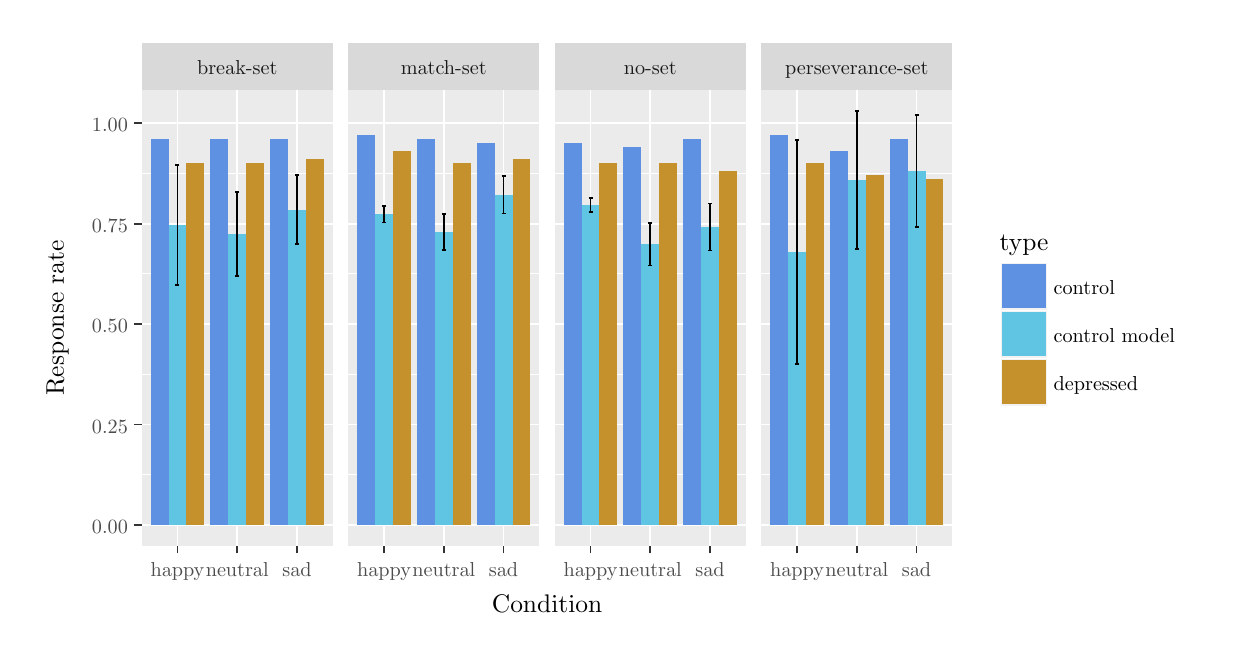
\begin{tikzpicture}[x=1pt,y=1pt]
\definecolor{fillColor}{RGB}{255,255,255}
\path[use as bounding box,fill=fillColor,fill opacity=0.00] (0,0) rectangle (433.62,216.81);
\begin{scope}
\path[clip] (  0.00,  0.00) rectangle (433.62,216.81);
\definecolor{drawColor}{RGB}{255,255,255}
\definecolor{fillColor}{RGB}{255,255,255}

\path[draw=drawColor,line width= 0.6pt,line join=round,line cap=round,fill=fillColor] (  0.00,  0.00) rectangle (433.62,216.81);
\end{scope}
\begin{scope}
\path[clip] ( 41.17, 29.59) rectangle (110.29,194.25);
\definecolor{fillColor}{gray}{0.92}

\path[fill=fillColor] ( 41.17, 29.59) rectangle (110.29,194.25);
\definecolor{drawColor}{RGB}{255,255,255}

\path[draw=drawColor,line width= 0.3pt,line join=round] ( 41.17, 55.22) --
	(110.29, 55.22);

\path[draw=drawColor,line width= 0.3pt,line join=round] ( 41.17, 91.52) --
	(110.29, 91.52);

\path[draw=drawColor,line width= 0.3pt,line join=round] ( 41.17,127.83) --
	(110.29,127.83);

\path[draw=drawColor,line width= 0.3pt,line join=round] ( 41.17,164.13) --
	(110.29,164.13);

\path[draw=drawColor,line width= 0.6pt,line join=round] ( 41.17, 37.07) --
	(110.29, 37.07);

\path[draw=drawColor,line width= 0.6pt,line join=round] ( 41.17, 73.37) --
	(110.29, 73.37);

\path[draw=drawColor,line width= 0.6pt,line join=round] ( 41.17,109.67) --
	(110.29,109.67);

\path[draw=drawColor,line width= 0.6pt,line join=round] ( 41.17,145.98) --
	(110.29,145.98);

\path[draw=drawColor,line width= 0.6pt,line join=round] ( 41.17,182.28) --
	(110.29,182.28);

\path[draw=drawColor,line width= 0.6pt,line join=round] ( 54.13, 29.59) --
	( 54.13,194.25);

\path[draw=drawColor,line width= 0.6pt,line join=round] ( 75.73, 29.59) --
	( 75.73,194.25);

\path[draw=drawColor,line width= 0.6pt,line join=round] ( 97.33, 29.59) --
	( 97.33,194.25);
\definecolor{fillColor}{RGB}{196,145,45}

\path[fill=fillColor] ( 57.37, 37.07) rectangle ( 63.85,167.76);
\definecolor{fillColor}{RGB}{95,197,226}

\path[fill=fillColor] ( 50.89, 37.07) rectangle ( 57.37,145.43);
\definecolor{fillColor}{RGB}{95,145,226}

\path[fill=fillColor] ( 44.41, 37.07) rectangle ( 50.89,176.47);
\definecolor{fillColor}{RGB}{196,145,45}

\path[fill=fillColor] ( 78.97, 37.07) rectangle ( 85.45,167.76);
\definecolor{fillColor}{RGB}{95,197,226}

\path[fill=fillColor] ( 72.49, 37.07) rectangle ( 78.97,142.23);
\definecolor{fillColor}{RGB}{95,145,226}

\path[fill=fillColor] ( 66.01, 37.07) rectangle ( 72.49,176.47);
\definecolor{fillColor}{RGB}{196,145,45}

\path[fill=fillColor] (100.57, 37.07) rectangle (107.05,169.21);
\definecolor{fillColor}{RGB}{95,197,226}

\path[fill=fillColor] ( 94.09, 37.07) rectangle (100.57,151.10);
\definecolor{fillColor}{RGB}{95,145,226}

\path[fill=fillColor] ( 87.61, 37.07) rectangle ( 94.09,176.47);
\definecolor{drawColor}{RGB}{0,0,0}

\path[draw=drawColor,line width= 0.6pt,line join=round] ( 53.41,167.13) --
	( 54.85,167.13);

\path[draw=drawColor,line width= 0.6pt,line join=round] ( 54.13,167.13) --
	( 54.13,123.73);

\path[draw=drawColor,line width= 0.6pt,line join=round] ( 53.41,123.73) --
	( 54.85,123.73);

\path[draw=drawColor,line width= 0.6pt,line join=round] ( 75.01,157.41) --
	( 76.45,157.41);

\path[draw=drawColor,line width= 0.6pt,line join=round] ( 75.73,157.41) --
	( 75.73,127.05);

\path[draw=drawColor,line width= 0.6pt,line join=round] ( 75.01,127.05) --
	( 76.45,127.05);

\path[draw=drawColor,line width= 0.6pt,line join=round] ( 96.61,163.68) --
	( 98.05,163.68);

\path[draw=drawColor,line width= 0.6pt,line join=round] ( 97.33,163.68) --
	( 97.33,138.53);

\path[draw=drawColor,line width= 0.6pt,line join=round] ( 96.61,138.53) --
	( 98.05,138.53);
\end{scope}
\begin{scope}
\path[clip] (115.79, 29.59) rectangle (184.92,194.25);
\definecolor{fillColor}{gray}{0.92}

\path[fill=fillColor] (115.79, 29.59) rectangle (184.92,194.25);
\definecolor{drawColor}{RGB}{255,255,255}

\path[draw=drawColor,line width= 0.3pt,line join=round] (115.79, 55.22) --
	(184.92, 55.22);

\path[draw=drawColor,line width= 0.3pt,line join=round] (115.79, 91.52) --
	(184.92, 91.52);

\path[draw=drawColor,line width= 0.3pt,line join=round] (115.79,127.83) --
	(184.92,127.83);

\path[draw=drawColor,line width= 0.3pt,line join=round] (115.79,164.13) --
	(184.92,164.13);

\path[draw=drawColor,line width= 0.6pt,line join=round] (115.79, 37.07) --
	(184.92, 37.07);

\path[draw=drawColor,line width= 0.6pt,line join=round] (115.79, 73.37) --
	(184.92, 73.37);

\path[draw=drawColor,line width= 0.6pt,line join=round] (115.79,109.67) --
	(184.92,109.67);

\path[draw=drawColor,line width= 0.6pt,line join=round] (115.79,145.98) --
	(184.92,145.98);

\path[draw=drawColor,line width= 0.6pt,line join=round] (115.79,182.28) --
	(184.92,182.28);

\path[draw=drawColor,line width= 0.6pt,line join=round] (128.76, 29.59) --
	(128.76,194.25);

\path[draw=drawColor,line width= 0.6pt,line join=round] (150.36, 29.59) --
	(150.36,194.25);

\path[draw=drawColor,line width= 0.6pt,line join=round] (171.96, 29.59) --
	(171.96,194.25);
\definecolor{fillColor}{RGB}{196,145,45}

\path[fill=fillColor] (132.00, 37.07) rectangle (138.48,172.11);
\definecolor{fillColor}{RGB}{95,197,226}

\path[fill=fillColor] (125.51, 37.07) rectangle (132.00,149.45);
\definecolor{fillColor}{RGB}{95,145,226}

\path[fill=fillColor] (119.03, 37.07) rectangle (125.51,177.92);
\definecolor{fillColor}{RGB}{196,145,45}

\path[fill=fillColor] (153.60, 37.07) rectangle (160.08,167.76);
\definecolor{fillColor}{RGB}{95,197,226}

\path[fill=fillColor] (147.12, 37.07) rectangle (153.60,143.03);
\definecolor{fillColor}{RGB}{95,145,226}

\path[fill=fillColor] (140.64, 37.07) rectangle (147.12,176.47);
\definecolor{fillColor}{RGB}{196,145,45}

\path[fill=fillColor] (175.20, 37.07) rectangle (181.68,169.21);
\definecolor{fillColor}{RGB}{95,197,226}

\path[fill=fillColor] (168.72, 37.07) rectangle (175.20,156.48);
\definecolor{fillColor}{RGB}{95,145,226}

\path[fill=fillColor] (162.24, 37.07) rectangle (168.72,175.02);
\definecolor{drawColor}{RGB}{0,0,0}

\path[draw=drawColor,line width= 0.6pt,line join=round] (128.04,152.46) --
	(129.48,152.46);

\path[draw=drawColor,line width= 0.6pt,line join=round] (128.76,152.46) --
	(128.76,146.43);

\path[draw=drawColor,line width= 0.6pt,line join=round] (128.04,146.43) --
	(129.48,146.43);

\path[draw=drawColor,line width= 0.6pt,line join=round] (149.64,149.58) --
	(151.08,149.58);

\path[draw=drawColor,line width= 0.6pt,line join=round] (150.36,149.58) --
	(150.36,136.49);

\path[draw=drawColor,line width= 0.6pt,line join=round] (149.64,136.49) --
	(151.08,136.49);

\path[draw=drawColor,line width= 0.6pt,line join=round] (171.24,163.26) --
	(172.68,163.26);

\path[draw=drawColor,line width= 0.6pt,line join=round] (171.96,163.26) --
	(171.96,149.69);

\path[draw=drawColor,line width= 0.6pt,line join=round] (171.24,149.69) --
	(172.68,149.69);
\end{scope}
\begin{scope}
\path[clip] (190.42, 29.59) rectangle (259.54,194.25);
\definecolor{fillColor}{gray}{0.92}

\path[fill=fillColor] (190.42, 29.59) rectangle (259.54,194.25);
\definecolor{drawColor}{RGB}{255,255,255}

\path[draw=drawColor,line width= 0.3pt,line join=round] (190.42, 55.22) --
	(259.54, 55.22);

\path[draw=drawColor,line width= 0.3pt,line join=round] (190.42, 91.52) --
	(259.54, 91.52);

\path[draw=drawColor,line width= 0.3pt,line join=round] (190.42,127.83) --
	(259.54,127.83);

\path[draw=drawColor,line width= 0.3pt,line join=round] (190.42,164.13) --
	(259.54,164.13);

\path[draw=drawColor,line width= 0.6pt,line join=round] (190.42, 37.07) --
	(259.54, 37.07);

\path[draw=drawColor,line width= 0.6pt,line join=round] (190.42, 73.37) --
	(259.54, 73.37);

\path[draw=drawColor,line width= 0.6pt,line join=round] (190.42,109.67) --
	(259.54,109.67);

\path[draw=drawColor,line width= 0.6pt,line join=round] (190.42,145.98) --
	(259.54,145.98);

\path[draw=drawColor,line width= 0.6pt,line join=round] (190.42,182.28) --
	(259.54,182.28);

\path[draw=drawColor,line width= 0.6pt,line join=round] (203.38, 29.59) --
	(203.38,194.25);

\path[draw=drawColor,line width= 0.6pt,line join=round] (224.98, 29.59) --
	(224.98,194.25);

\path[draw=drawColor,line width= 0.6pt,line join=round] (246.58, 29.59) --
	(246.58,194.25);
\definecolor{fillColor}{RGB}{196,145,45}

\path[fill=fillColor] (206.62, 37.07) rectangle (213.10,167.76);
\definecolor{fillColor}{RGB}{95,197,226}

\path[fill=fillColor] (200.14, 37.07) rectangle (206.62,152.68);
\definecolor{fillColor}{RGB}{95,145,226}

\path[fill=fillColor] (193.66, 37.07) rectangle (200.14,175.02);
\definecolor{fillColor}{RGB}{196,145,45}

\path[fill=fillColor] (228.22, 37.07) rectangle (234.70,167.76);
\definecolor{fillColor}{RGB}{95,197,226}

\path[fill=fillColor] (221.74, 37.07) rectangle (228.22,138.48);
\definecolor{fillColor}{RGB}{95,145,226}

\path[fill=fillColor] (215.26, 37.07) rectangle (221.74,173.57);
\definecolor{fillColor}{RGB}{196,145,45}

\path[fill=fillColor] (249.82, 37.07) rectangle (256.30,164.85);
\definecolor{fillColor}{RGB}{95,197,226}

\path[fill=fillColor] (243.34, 37.07) rectangle (249.82,144.74);
\definecolor{fillColor}{RGB}{95,145,226}

\path[fill=fillColor] (236.86, 37.07) rectangle (243.34,176.47);
\definecolor{drawColor}{RGB}{0,0,0}

\path[draw=drawColor,line width= 0.6pt,line join=round] (202.66,155.20) --
	(204.10,155.20);

\path[draw=drawColor,line width= 0.6pt,line join=round] (203.38,155.20) --
	(203.38,150.15);

\path[draw=drawColor,line width= 0.6pt,line join=round] (202.66,150.15) --
	(204.10,150.15);

\path[draw=drawColor,line width= 0.6pt,line join=round] (224.26,146.13) --
	(225.70,146.13);

\path[draw=drawColor,line width= 0.6pt,line join=round] (224.98,146.13) --
	(224.98,130.83);

\path[draw=drawColor,line width= 0.6pt,line join=round] (224.26,130.83) --
	(225.70,130.83);

\path[draw=drawColor,line width= 0.6pt,line join=round] (245.86,153.25) --
	(247.30,153.25);

\path[draw=drawColor,line width= 0.6pt,line join=round] (246.58,153.25) --
	(246.58,136.23);

\path[draw=drawColor,line width= 0.6pt,line join=round] (245.86,136.23) --
	(247.30,136.23);
\end{scope}
\begin{scope}
\path[clip] (265.04, 29.59) rectangle (334.16,194.25);
\definecolor{fillColor}{gray}{0.92}

\path[fill=fillColor] (265.04, 29.59) rectangle (334.16,194.25);
\definecolor{drawColor}{RGB}{255,255,255}

\path[draw=drawColor,line width= 0.3pt,line join=round] (265.04, 55.22) --
	(334.16, 55.22);

\path[draw=drawColor,line width= 0.3pt,line join=round] (265.04, 91.52) --
	(334.16, 91.52);

\path[draw=drawColor,line width= 0.3pt,line join=round] (265.04,127.83) --
	(334.16,127.83);

\path[draw=drawColor,line width= 0.3pt,line join=round] (265.04,164.13) --
	(334.16,164.13);

\path[draw=drawColor,line width= 0.6pt,line join=round] (265.04, 37.07) --
	(334.16, 37.07);

\path[draw=drawColor,line width= 0.6pt,line join=round] (265.04, 73.37) --
	(334.16, 73.37);

\path[draw=drawColor,line width= 0.6pt,line join=round] (265.04,109.67) --
	(334.16,109.67);

\path[draw=drawColor,line width= 0.6pt,line join=round] (265.04,145.98) --
	(334.16,145.98);

\path[draw=drawColor,line width= 0.6pt,line join=round] (265.04,182.28) --
	(334.16,182.28);

\path[draw=drawColor,line width= 0.6pt,line join=round] (278.00, 29.59) --
	(278.00,194.25);

\path[draw=drawColor,line width= 0.6pt,line join=round] (299.60, 29.59) --
	(299.60,194.25);

\path[draw=drawColor,line width= 0.6pt,line join=round] (321.20, 29.59) --
	(321.20,194.25);
\definecolor{fillColor}{RGB}{196,145,45}

\path[fill=fillColor] (281.24, 37.07) rectangle (287.72,167.76);
\definecolor{fillColor}{RGB}{95,197,226}

\path[fill=fillColor] (274.76, 37.07) rectangle (281.24,135.74);
\definecolor{fillColor}{RGB}{95,145,226}

\path[fill=fillColor] (268.28, 37.07) rectangle (274.76,177.92);
\definecolor{fillColor}{RGB}{196,145,45}

\path[fill=fillColor] (302.84, 37.07) rectangle (309.32,163.40);
\definecolor{fillColor}{RGB}{95,197,226}

\path[fill=fillColor] (296.36, 37.07) rectangle (302.84,161.74);
\definecolor{fillColor}{RGB}{95,145,226}

\path[fill=fillColor] (289.88, 37.07) rectangle (296.36,172.11);
\definecolor{fillColor}{RGB}{196,145,45}

\path[fill=fillColor] (324.44, 37.07) rectangle (330.92,161.95);
\definecolor{fillColor}{RGB}{95,197,226}

\path[fill=fillColor] (317.96, 37.07) rectangle (324.44,165.04);
\definecolor{fillColor}{RGB}{95,145,226}

\path[fill=fillColor] (311.48, 37.07) rectangle (317.96,176.47);
\definecolor{drawColor}{RGB}{0,0,0}

\path[draw=drawColor,line width= 0.6pt,line join=round] (277.28,176.14) --
	(278.72,176.14);

\path[draw=drawColor,line width= 0.6pt,line join=round] (278.00,176.14) --
	(278.00, 95.34);

\path[draw=drawColor,line width= 0.6pt,line join=round] (277.28, 95.34) --
	(278.72, 95.34);

\path[draw=drawColor,line width= 0.6pt,line join=round] (298.88,186.76) --
	(300.32,186.76);

\path[draw=drawColor,line width= 0.6pt,line join=round] (299.60,186.76) --
	(299.60,136.72);

\path[draw=drawColor,line width= 0.6pt,line join=round] (298.88,136.72) --
	(300.32,136.72);

\path[draw=drawColor,line width= 0.6pt,line join=round] (320.48,185.34) --
	(321.92,185.34);

\path[draw=drawColor,line width= 0.6pt,line join=round] (321.20,185.34) --
	(321.20,144.75);

\path[draw=drawColor,line width= 0.6pt,line join=round] (320.48,144.75) --
	(321.92,144.75);
\end{scope}
\begin{scope}
\path[clip] ( 41.17,194.25) rectangle (110.29,211.31);
\definecolor{fillColor}{gray}{0.85}

\path[fill=fillColor] ( 41.17,194.25) rectangle (110.29,211.31);
\definecolor{drawColor}{gray}{0.10}

\node[text=drawColor,anchor=base,inner sep=0pt, outer sep=0pt, scale=  0.73] at ( 75.73,199.75) {break-set};
\end{scope}
\begin{scope}
\path[clip] (115.79,194.25) rectangle (184.92,211.31);
\definecolor{fillColor}{gray}{0.85}

\path[fill=fillColor] (115.79,194.25) rectangle (184.92,211.31);
\definecolor{drawColor}{gray}{0.10}

\node[text=drawColor,anchor=base,inner sep=0pt, outer sep=0pt, scale=  0.73] at (150.36,199.75) {match-set};
\end{scope}
\begin{scope}
\path[clip] (190.42,194.25) rectangle (259.54,211.31);
\definecolor{fillColor}{gray}{0.85}

\path[fill=fillColor] (190.42,194.25) rectangle (259.54,211.31);
\definecolor{drawColor}{gray}{0.10}

\node[text=drawColor,anchor=base,inner sep=0pt, outer sep=0pt, scale=  0.73] at (224.98,199.75) {no-set};
\end{scope}
\begin{scope}
\path[clip] (265.04,194.25) rectangle (334.16,211.31);
\definecolor{fillColor}{gray}{0.85}

\path[fill=fillColor] (265.04,194.25) rectangle (334.16,211.31);
\definecolor{drawColor}{gray}{0.10}

\node[text=drawColor,anchor=base,inner sep=0pt, outer sep=0pt, scale=  0.73] at (299.60,199.75) {perseverance-set};
\end{scope}
\begin{scope}
\path[clip] (  0.00,  0.00) rectangle (433.62,216.81);
\definecolor{drawColor}{gray}{0.20}

\path[draw=drawColor,line width= 0.6pt,line join=round] ( 54.13, 26.84) --
	( 54.13, 29.59);

\path[draw=drawColor,line width= 0.6pt,line join=round] ( 75.73, 26.84) --
	( 75.73, 29.59);

\path[draw=drawColor,line width= 0.6pt,line join=round] ( 97.33, 26.84) --
	( 97.33, 29.59);
\end{scope}
\begin{scope}
\path[clip] (  0.00,  0.00) rectangle (433.62,216.81);
\definecolor{drawColor}{gray}{0.30}

\node[text=drawColor,anchor=base,inner sep=0pt, outer sep=0pt, scale=  0.73] at ( 54.13, 18.58) {happy};

\node[text=drawColor,anchor=base,inner sep=0pt, outer sep=0pt, scale=  0.73] at ( 75.73, 18.58) {neutral};

\node[text=drawColor,anchor=base,inner sep=0pt, outer sep=0pt, scale=  0.73] at ( 97.33, 18.58) {sad};
\end{scope}
\begin{scope}
\path[clip] (  0.00,  0.00) rectangle (433.62,216.81);
\definecolor{drawColor}{gray}{0.20}

\path[draw=drawColor,line width= 0.6pt,line join=round] (128.76, 26.84) --
	(128.76, 29.59);

\path[draw=drawColor,line width= 0.6pt,line join=round] (150.36, 26.84) --
	(150.36, 29.59);

\path[draw=drawColor,line width= 0.6pt,line join=round] (171.96, 26.84) --
	(171.96, 29.59);
\end{scope}
\begin{scope}
\path[clip] (  0.00,  0.00) rectangle (433.62,216.81);
\definecolor{drawColor}{gray}{0.30}

\node[text=drawColor,anchor=base,inner sep=0pt, outer sep=0pt, scale=  0.73] at (128.76, 18.58) {happy};

\node[text=drawColor,anchor=base,inner sep=0pt, outer sep=0pt, scale=  0.73] at (150.36, 18.58) {neutral};

\node[text=drawColor,anchor=base,inner sep=0pt, outer sep=0pt, scale=  0.73] at (171.96, 18.58) {sad};
\end{scope}
\begin{scope}
\path[clip] (  0.00,  0.00) rectangle (433.62,216.81);
\definecolor{drawColor}{gray}{0.20}

\path[draw=drawColor,line width= 0.6pt,line join=round] (203.38, 26.84) --
	(203.38, 29.59);

\path[draw=drawColor,line width= 0.6pt,line join=round] (224.98, 26.84) --
	(224.98, 29.59);

\path[draw=drawColor,line width= 0.6pt,line join=round] (246.58, 26.84) --
	(246.58, 29.59);
\end{scope}
\begin{scope}
\path[clip] (  0.00,  0.00) rectangle (433.62,216.81);
\definecolor{drawColor}{gray}{0.30}

\node[text=drawColor,anchor=base,inner sep=0pt, outer sep=0pt, scale=  0.73] at (203.38, 18.58) {happy};

\node[text=drawColor,anchor=base,inner sep=0pt, outer sep=0pt, scale=  0.73] at (224.98, 18.58) {neutral};

\node[text=drawColor,anchor=base,inner sep=0pt, outer sep=0pt, scale=  0.73] at (246.58, 18.58) {sad};
\end{scope}
\begin{scope}
\path[clip] (  0.00,  0.00) rectangle (433.62,216.81);
\definecolor{drawColor}{gray}{0.20}

\path[draw=drawColor,line width= 0.6pt,line join=round] (278.00, 26.84) --
	(278.00, 29.59);

\path[draw=drawColor,line width= 0.6pt,line join=round] (299.60, 26.84) --
	(299.60, 29.59);

\path[draw=drawColor,line width= 0.6pt,line join=round] (321.20, 26.84) --
	(321.20, 29.59);
\end{scope}
\begin{scope}
\path[clip] (  0.00,  0.00) rectangle (433.62,216.81);
\definecolor{drawColor}{gray}{0.30}

\node[text=drawColor,anchor=base,inner sep=0pt, outer sep=0pt, scale=  0.73] at (278.00, 18.58) {happy};

\node[text=drawColor,anchor=base,inner sep=0pt, outer sep=0pt, scale=  0.73] at (299.60, 18.58) {neutral};

\node[text=drawColor,anchor=base,inner sep=0pt, outer sep=0pt, scale=  0.73] at (321.20, 18.58) {sad};
\end{scope}
\begin{scope}
\path[clip] (  0.00,  0.00) rectangle (433.62,216.81);
\definecolor{drawColor}{gray}{0.30}

\node[text=drawColor,anchor=base east,inner sep=0pt, outer sep=0pt, scale=  0.73] at ( 36.22, 34.04) {0.00};

\node[text=drawColor,anchor=base east,inner sep=0pt, outer sep=0pt, scale=  0.73] at ( 36.22, 70.34) {0.25};

\node[text=drawColor,anchor=base east,inner sep=0pt, outer sep=0pt, scale=  0.73] at ( 36.22,106.64) {0.50};

\node[text=drawColor,anchor=base east,inner sep=0pt, outer sep=0pt, scale=  0.73] at ( 36.22,142.95) {0.75};

\node[text=drawColor,anchor=base east,inner sep=0pt, outer sep=0pt, scale=  0.73] at ( 36.22,179.25) {1.00};
\end{scope}
\begin{scope}
\path[clip] (  0.00,  0.00) rectangle (433.62,216.81);
\definecolor{drawColor}{gray}{0.20}

\path[draw=drawColor,line width= 0.6pt,line join=round] ( 38.42, 37.07) --
	( 41.17, 37.07);

\path[draw=drawColor,line width= 0.6pt,line join=round] ( 38.42, 73.37) --
	( 41.17, 73.37);

\path[draw=drawColor,line width= 0.6pt,line join=round] ( 38.42,109.67) --
	( 41.17,109.67);

\path[draw=drawColor,line width= 0.6pt,line join=round] ( 38.42,145.98) --
	( 41.17,145.98);

\path[draw=drawColor,line width= 0.6pt,line join=round] ( 38.42,182.28) --
	( 41.17,182.28);
\end{scope}
\begin{scope}
\path[clip] (  0.00,  0.00) rectangle (433.62,216.81);
\definecolor{drawColor}{RGB}{0,0,0}

\node[text=drawColor,anchor=base,inner sep=0pt, outer sep=0pt, scale=  0.92] at (187.67,  5.50) {Condition};
\end{scope}
\begin{scope}
\path[clip] (  0.00,  0.00) rectangle (433.62,216.81);
\definecolor{drawColor}{RGB}{0,0,0}

\node[text=drawColor,rotate= 90.00,anchor=base,inner sep=0pt, outer sep=0pt, scale=  0.92] at ( 13.08,111.92) {Response rate};
\end{scope}
\begin{scope}
\path[clip] (  0.00,  0.00) rectangle (433.62,216.81);
\definecolor{fillColor}{RGB}{255,255,255}

\path[fill=fillColor] (345.54, 74.25) rectangle (428.12,149.58);
\end{scope}
\begin{scope}
\path[clip] (  0.00,  0.00) rectangle (433.62,216.81);
\definecolor{drawColor}{RGB}{0,0,0}

\node[text=drawColor,anchor=base west,inner sep=0pt, outer sep=0pt, scale=  0.92] at (351.23,136.32) {type};
\end{scope}
\begin{scope}
\path[clip] (  0.00,  0.00) rectangle (433.62,216.81);
\definecolor{drawColor}{RGB}{255,255,255}
\definecolor{fillColor}{gray}{0.95}

\path[draw=drawColor,line width= 0.6pt,line join=round,line cap=round,fill=fillColor] (351.23,114.63) rectangle (368.58,131.98);
\end{scope}
\begin{scope}
\path[clip] (  0.00,  0.00) rectangle (433.62,216.81);
\definecolor{fillColor}{RGB}{95,145,226}

\path[fill=fillColor] (351.94,115.35) rectangle (367.86,131.27);
\end{scope}
\begin{scope}
\path[clip] (  0.00,  0.00) rectangle (433.62,216.81);
\definecolor{drawColor}{RGB}{255,255,255}
\definecolor{fillColor}{gray}{0.95}

\path[draw=drawColor,line width= 0.6pt,line join=round,line cap=round,fill=fillColor] (351.23, 97.29) rectangle (368.58,114.63);
\end{scope}
\begin{scope}
\path[clip] (  0.00,  0.00) rectangle (433.62,216.81);
\definecolor{fillColor}{RGB}{95,197,226}

\path[fill=fillColor] (351.94, 98.00) rectangle (367.86,113.92);
\end{scope}
\begin{scope}
\path[clip] (  0.00,  0.00) rectangle (433.62,216.81);
\definecolor{drawColor}{RGB}{255,255,255}
\definecolor{fillColor}{gray}{0.95}

\path[draw=drawColor,line width= 0.6pt,line join=round,line cap=round,fill=fillColor] (351.23, 79.94) rectangle (368.58, 97.29);
\end{scope}
\begin{scope}
\path[clip] (  0.00,  0.00) rectangle (433.62,216.81);
\definecolor{fillColor}{RGB}{196,145,45}

\path[fill=fillColor] (351.94, 80.66) rectangle (367.86, 96.58);
\end{scope}
\begin{scope}
\path[clip] (  0.00,  0.00) rectangle (433.62,216.81);
\definecolor{drawColor}{RGB}{0,0,0}

\node[text=drawColor,anchor=base west,inner sep=0pt, outer sep=0pt, scale=  0.73] at (370.74,120.28) {control};
\end{scope}
\begin{scope}
\path[clip] (  0.00,  0.00) rectangle (433.62,216.81);
\definecolor{drawColor}{RGB}{0,0,0}

\node[text=drawColor,anchor=base west,inner sep=0pt, outer sep=0pt, scale=  0.73] at (370.74,102.93) {control model};
\end{scope}
\begin{scope}
\path[clip] (  0.00,  0.00) rectangle (433.62,216.81);
\definecolor{drawColor}{RGB}{0,0,0}

\node[text=drawColor,anchor=base west,inner sep=0pt, outer sep=0pt, scale=  0.73] at (370.74, 85.59) {depressed};
\end{scope}
\end{tikzpicture}
